\documentclass{article}

\usepackage{graphicx}
\usepackage{tikz}
\usepackage{tikzsymbols}
\usetikzlibrary{calc,patterns,shapes.geometric}
\pagestyle{empty}
\usepackage[margin=0pt]{geometry}
\geometry{papersize={14in,12in}}

\def\centerarc[#1](#2)(#3:#4:#5){\draw[#1] ($(#2)+({#5*cos(#3)},{#5*sin(#3)})$) arc (#3:#4:#5);}

\begin{document}
	\begin{figure}
		\centering
		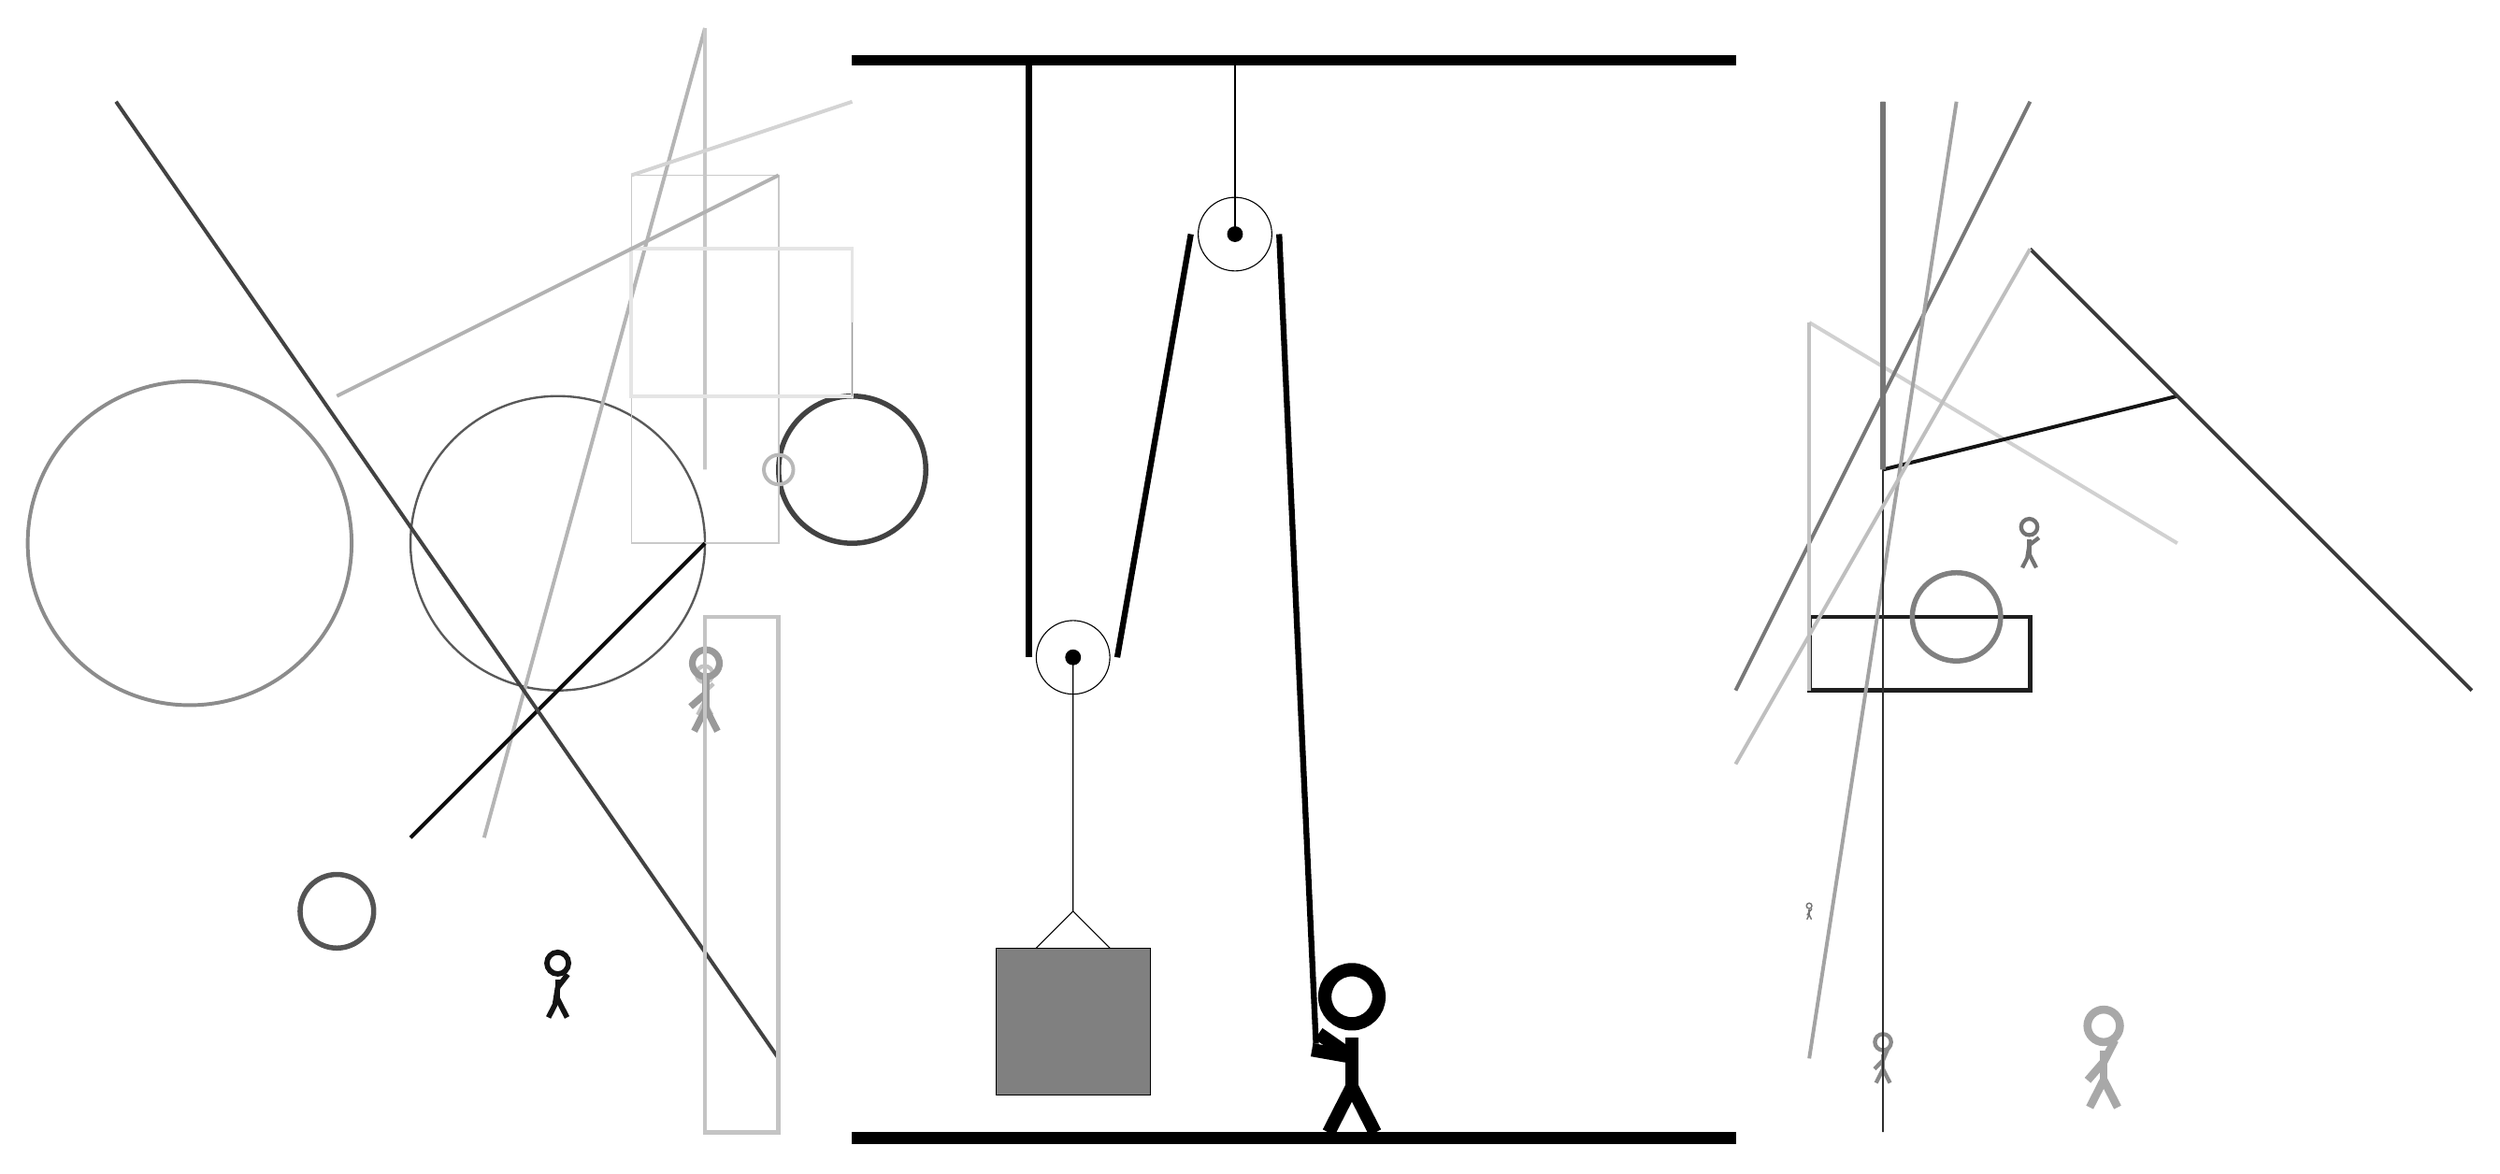
\begin{tikzpicture}
			%%%%% START %%%%%
			
			\draw[fill=black] (-2, 11.5) rectangle (10, 11.625);
			
			\draw (3.2, 9.2) circle (0.5);
			\draw[fill=black] (3.2, 9.2) circle (0.1);
			\draw[thick] (3.2, 9.2) -- (3.2, 11.5);
			
			\draw (1, 3.45) circle (0.5);
			\draw[fill=black] (1, 3.45) circle (0.1);
			
			\draw (1, 3.45) -- (1, 0.0) -- (0.5, -0.5);
			\draw (1, 0.0) -- (1.5, -0.5);
			\draw[fill=black!50] (-0.05, -0.5) rectangle (2.05, -2.5);
			
			\draw[line width=0.8mm] (0.4, 11.5) -- (0.4, 3.45);
			\centerarc[line width=0.8mm](1, 3.45)(180:360:0.6);
			\draw[line width=0.8mm](1.6, 3.45) -- (2.6, 9.2);
			\centerarc[line width=0.8mm](3.2, 9.2)(0:180:0.6);
			\draw[line width=0.8mm](3.8, 9.2) -- (4.3, -1.8);
			
			\node at (4.7, -1.9) {\Strichmaxerl[10][-35][170]};
			
			\draw[line width=0.6mm, color=black!88] (11, 3) rectangle (14, 4);
			
			\draw[line width=0.5mm, color=black!18](11, 8) -- (16, 5);
			\draw[line width=0.6mm, color=black!75] (12, 7) rectangle (12, 11);
			\draw [line width=0.7mm, color=black!74](-2, 6) circle (1.0);
			
			\draw[line width=0.5mm, color=black!53](10, 3) -- (14, 11);
			
			\draw [line width=0.3mm, color=black!65](-6, 5) circle (2.0);
			
			\draw[line width=0.5mm, color=black!92](12, 6) -- (16, 7);
			\draw[line width=0.2mm, color=black!21] (-3, 10) rectangle (-5, 5);
			\node[line width=0.5mm, color=black!24] at (-4, 3) {\Strichmaxerl[3][57][44]};
			\draw[line width=0.5mm, color=black!24](11, 8) -- (11, 3);
			\draw[line width=0.5mm, color=black!36](13, 11) -- (11, -2);
			\draw[line width=0.5mm, color=black!29](-4, 12) -- (-7, 1);
			\draw[line width=0.6mm, color=black!22] (-4, 12) rectangle (-4, 6);
			
			\node[line width=0.7mm, color=black!55] at (14, 5) {\Strichmaxerl[3][81][37]};
			\node[line width=0.7mm, color=black!54] at (11, 0) {\Strichmaxerl[1][59][47]};
			\draw[line width=0.5mm, color=black!10] (-2, 7) rectangle (-5, 9);
			\draw[line width=0.5mm, color=black!30](-3, 10) -- (-9, 7);
			\node[line width=0.7mm, color=black!46] at (12, -2) {\Strichmaxerl[3][46][67]};
			\draw[line width=0.7mm, color=black!54] (12, 11) rectangle (12, 6);
			
			\draw [line width=0.7mm, color=black!67](-9, 0) circle (0.5);
			\node[line width=0.3mm, color=black!40] at (-4, 3) {\Strichmaxerl[5][41][90]};
			
			\draw[line width=0.5mm, color=black!77](14, 9) -- (20, 3);
			\draw[line width=0.5mm, color=black!17](-2, 11) -- (-5, 10);
			\draw[line width=0.2mm, color=black!82] (12, -3) rectangle (12, 6);
			\draw[line width=0.5mm, color=black!95](-4, 5) -- (-8, 1);
			
			\node[line width=0.4mm, color=black!34] at (15, -2) {\Strichmaxerl[6][49][63]};
			\draw [line width=0.5mm, color=black!28](-3, 6) circle (0.2);
			\draw [line width=0.5mm, color=black!45](-11, 5) circle (2.2);
			\draw[line width=0.5mm, color=black!74](-3, -2) -- (-12, 11);
			\draw[line width=0.2mm, color=black!40] (-2, 7) rectangle (-2, 8);
			\draw[line width=0.5mm, color=black!25](14, 9) -- (10, 2);
			
			\draw[line width=0.6mm, color=black!23] (-3, 4) rectangle (-4, -3);
			\draw [line width=0.7mm, color=black!50](13, 4) circle (0.6);
			\node[line width=0.4mm, color=black!92] at (-6, -1) {\Strichmaxerl[4][81][52]};
			
			\draw[fill=black] (-2, -3) rectangle (10, -3.15);
			
			%%%%% END %%%%%
		\end{tikzpicture}
	\end{figure}	
\end{document}